\begin{titlepage}
    \centering
    
    \begin{tikzpicture}[scale=1.0, thick]
        \newcommand{\xoff}{-3}
        \newcommand{\yoff}{-3}
        \newcommand{\xlen}{10}
        \newcommand{\ylen}{11}
        \newcommand{\ylene}{10}

        \newcommand{\esize}{0.2} % radius: electron
        \newcommand{\ediam}{0.4} % diameter: electron
        \newcommand{\csize}{0.3} % radius: cation
        \newcommand{\cdiam}{0.6} % diameter: cation 
        \newcommand{\asize}{\csize} %radius: anions 
        \newcommand{\adiam}{\cdiam} %diameter: anions 
        \newcommand{\ssize}{0.4} %radius: solvent
        \newcommand{\sdiam}{0.8} %diameter: solvent

        \newcommand{\xihp}{\csize} % x position: Inner Helmoltz Potential
        \newcommand{\xohp}{2}      % x position: Outer Helmoltz Potential


        \coordinate (Um) at (-\esize, 4);  % Potential of metal
        \coordinate (Uihp) at (\csize, 6); % Potential IHP
        \coordinate (Uohp) at (\xohp, 5); % Potential OHP
        \coordinate (Udiff) at (\xlen-0.2, 0); % Potential OHP


        \draw[thick, arrows=->] (\xoff, 0) -- (\xlen,0) node[below, anchor=north, yshift=-0.2cm] {\Large \bf Distance x}; % x axis

        % Metal htach
        \draw[draw=none,pattern={Lines[angle=45,distance={0.5cm},xshift=.1pt]}] (\xoff, 0) rectangle (0,\ylen);
        \node[fill=white] at (\xoff/2.0, \ylen/2.0) {\Large METAL};
        \draw[thick, arrows=->] (0, \yoff) -- (0,\ylen) node[left, anchor=east, rotate=90, yshift=+1cm, fill=white] {\color{red}\Large \bf Potential $\Phi$}; % y axis
        
        % IHP/OHP/diffuse layer
        \draw[dashed] (\xihp, -1) -- (\xihp, \ylen+1) node [at start, yshift=-0.2cm] {IHP};
        \draw[dashed] (\xohp, -1) -- (\xohp, \ylen+1) node [at start, yshift=-0.2cm] {OHP};
        \node[anchor=south west] at (\xohp+3, \ylen-0.5) {Diffuse Layer};
        
        % negative charges in metal
        \foreach \i [evaluate=\i as \y using \i+\esize] in {0,\ediam,...,\ylene}
        {
            \filldraw[fill=white] (-\esize, \y) circle (\esize) node {-};
        }
        
        % solvent adsorbed
        \foreach \i [evaluate=\i as \y using \i+\ssize] in {0, \sdiam,...,\ylen}
        {
            \draw[fill=white] (+\ssize, \y) circle (\ssize) node {s};
        }
        
        % cations adsorbed on surface in electrolyte
        \foreach \i [evaluate=\i as \y using \i+\csize] in {2, 6, 10}
        {
            \draw[fill=white] (+\csize, \y) circle (\csize) node {+};
        }



        % solvated anions
        \foreach \x/\y/\r in {\xohp/2/0, \xohp/6/10, \xohp/10/20, %
                              \xohp+3/3/35,%
                              \xohp+3/8/45,%
                              \xohp+6/4/65,%
                              \xohp+6/9/-45}
        {
            \foreach \a in {0,72,...,360}
            {
                \draw[fill=white] (\x,\y) circle (\asize) node {-};
                \draw[fill=white] ($(\x,\y)+(\a+\r:\asize+\ssize)$) circle (\ssize) node {s};
            }
        }

        \node at (\xohp+7,6) {Solvated anions};
        \draw[red, line width=0.075cm] (Um) -- (Uihp) -- (Uohp) to[out=-90, in=180]  (Udiff);

    \end{tikzpicture}
    \vspace{1cm}
    
    {\Huge \textsc{Electrochemistry}\par}
    \hrulefill \par
    {\large Milan Skocic, PhD.}
    

    \vfill
    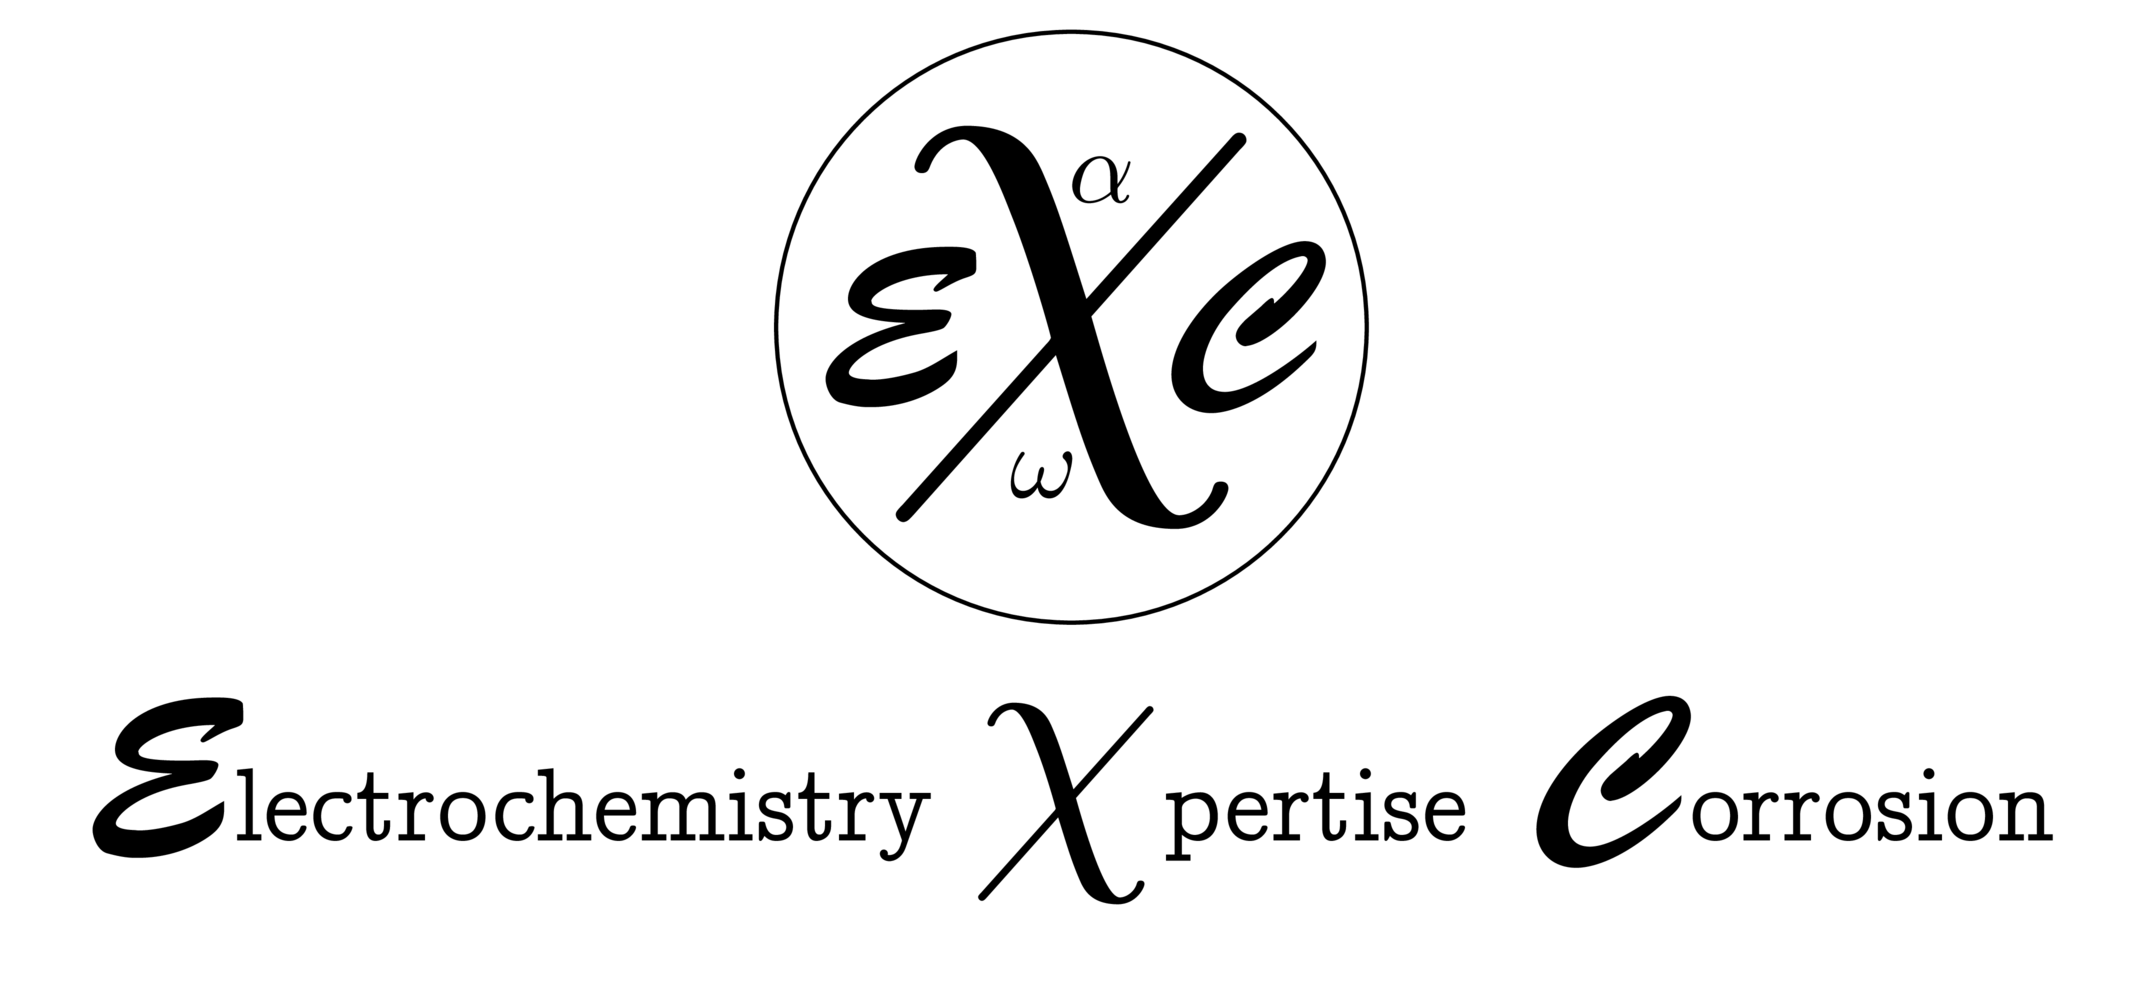
\includegraphics[width=0.65\textwidth]{full_bw.png}


\end{titlepage}
